% monet.tex
%
% Aetf <aetf@unlimitedcodeworks.xyz>
% Copyright 2016 Aetf <aetf@unlimitedcodeworks.xyz>
%
% multiple1902 <multiple1902@gmail.com>
% Copyright 2011~2012, multiple1902 (Weisi Dai)
%
% Project Home: https://github.com/Aetf/xjtuthesis
%
% It is strongly recommended that you read documentations located at
%   https://github.com/Aetf/xjtuthesis/wiki
% in advance of your compilation if you have not read them before.
%
% This work may be distributed and/or modified under the
% conditions of the LaTeX Project Public License, either version 1.3
% of this license or (at your option) any later version.
% The latest version of this license is in
%   http://www.latex-project.org/lppl.txt
% and version 1.3 or later is part of all distributions of LaTeX
% version 2005/12/01 or later.
%
% This work has the LPPL maintenance status `maintained'.
%
% The Current Maintainer of this work is Aetf.
%
% Almost all text in this file are taken from Chinese Wikipedia at
%   https://zh.wikipedia.org/zh/克洛德·莫奈
% or 
%   https://zh.wikipedia.org/wiki/%E5%85%8B%E6%B4%9B%E5%BE%B7%C2%B7%E8%8E%AB%E5%A5%88
% and are released under Creative Commons Attribution-Share Alike License 3.0
% which can be found at 
%   https://en.wikipedia.org/wiki/Wikipedia:Text_of_Creative_Commons_Attribution-ShareAlike_3.0_Unported_License
%
\chapter{克洛德·莫奈}
\echapter{Claude Monet}

\begin{quotation}
    编者注:本章内容取自「维基百科,自由的百科全书」,并以创作共用「署名-相同方式共享」授权重新发布。\xjtuthesis 第一版的开发代号为~Monet。
\end{quotation}

    克洛德·莫奈\footnote{法语:Claude Monet,1840年11月14日 --- 1926年12月5日}(图\ref{fig:claude-monet}),法国画家,印象派代表人物和创始人之一。印象出自其代表作《印象·日出》的标题。

    \begin{figure}[h!]
      \centering
      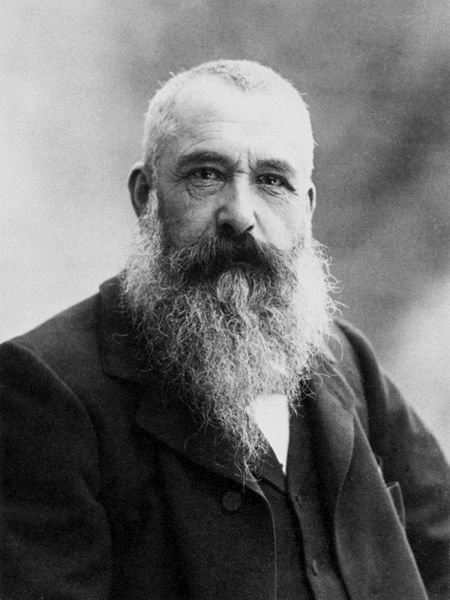
\includegraphics[width=6.67cm]{450px-Claude_Monet_1899_Nadar_crop.jpg}
      \caption{Claude Monet (公有领域)}
      \label{fig:claude-monet}
    \end{figure}

    莫奈是法国最重要的画家之一,印象派的理论和实践大部份都有他的推广。莫奈擅长光与影的实验与表现技法。他最重要的风格是改变了阴影和轮廓线的画法,在莫奈的画作中看不到非常明确的阴影,也看不到突显或平涂式的轮廓线。除此之外,莫奈对于色彩的运用相当细腻,他用许多相同主题的画作来实验色彩与光完美的表达。莫奈曾长期探索光色与空气的表现效果,常常在不同的时间和光线下,对同一对象作多幅的描绘,从自然的光色变幻中抒发瞬间的感觉。

    \section{早年生涯}
    \esection{Early Years}

        莫奈1840年11月14日出生于法国巴黎45街拉菲特第九郡,是阿道夫和路易斯的第二个儿子。他的父母都是第二代的巴黎人。1841年5月20日,他在当地的巴黎圣母院教区教堂受洗。在全家搬到了在诺曼底、位于塞纳河口北岸的勒阿弗尔\footnote{Le Havre}。他的父亲希望他继承家里的杂货店,但莫奈则想成为一个艺术家。他的母亲是一名歌手。

        1851年4月1日起,莫奈进入勒阿弗尔艺术中学。他的木炭漫画开价十到二十法郎,因此为当地人熟知。莫奈跟从雅克-弗兰柯伊斯·奥查德学习了最初的绘画课程,而后者是雅克-路易·大卫。在诺曼底的海滩上,他遇到了艺术家欧仁·布丹\footnote{Eugene Boudin},他后来成了莫奈的良师益友并教授他学会画油画。布丹教了莫奈绘画上的「空气」技法。

        1857年1月28日,他的母亲去世了。因此他从16岁起,离开学校,和丧偶无子女的姨妈玛丽-让娜·列卡德\footnote{Marie-Jeanne Lecadre}居住。

    \section{在巴黎}
    \esection{In Paris}

        当莫奈来到巴黎卢浮宫,他亲眼看到许多画家在模仿著名艺术家的作品。于是,随身携带着颜料和工具的他便坐在一扇窗户旁开始画他所看到的东西。莫奈在法国居住了数年,并与其他年轻画家会面。其中爱德华·马奈成为了他的好朋友,并且也是印象派画家。

        \begin{figure}[h!]
          \centering
          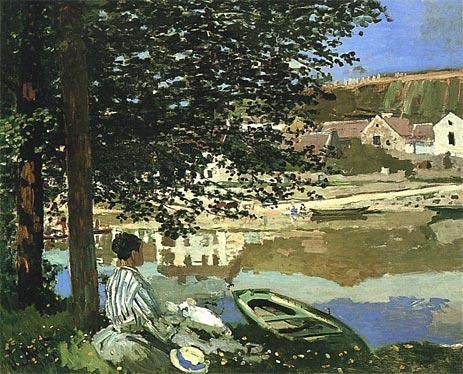
\includegraphics[width=6.67cm]{Claude_Monet_River_Scene_at_Bennecourt_Seine.jpg}
          \caption{\textit{On the Bank of the Seine, Bennecourt} (公有领域)}
          \label{fig:on-the-bank-of-the-seine}
        \end{figure}

        莫奈在阿尔及利亚当了两年兵\footnote{1860年 --- 1862年},在他服役七年的合同到期之前,因为伤寒,莫奈的姑妈Lecadre夫人将他从部队解脱出来,让他去完成大学的艺术课程。这可能是在他认识的荷兰画家Johan~Barthold~Jongkind的干预下完成的。

        因为大学的传统艺术教育让他觉醒,1862年莫奈在巴黎加入了夏尔·格莱尔\footnote{Charles Gleyre}画室。在那里他结认了皮耶-奥古斯特·雷诺阿、弗雷德里克·巴齐耶\footnote{Frederic Bazille}以及阿尔弗雷德·西斯莉\footnote{Alfred Sisley}。他们共同创造了一种新的艺术手法,即在户外和自然光线下用浓厚的油彩作画,后来被称为印象派。

        1866年,他以卡米耶·东西厄\footnote{Camille Doncieux}为模特创作了《绿衣女人》\footnote{\textit{The Woman in the Green Dress}}。这件作品使他受到承认。卡米耶也是他次年作品《花园中的女人》中的模特,还出现在他1868年在塞纳河岸上绘制的《塞纳河岸》中。不久之后,卡米耶即怀孕并生下了他们的第一个孩子让\footnote{Jean}。

    \section{普法战争,印象派,阿尔}
    \esection{Franco-Prussian War, Impressionism, and Argenteuil}

        在普法战争\footnote{Franco-Prussian War,1870年 --- 1871年}期间,莫奈于1870年9月来到英国避难。在那里他学习约翰·康斯太布尔和J·M·W·透纳\footnote{J.M.W.Turner}的作品。他们的作品激发了莫奈对色彩研究方面的创新。1871年春天,皇家艺术学院拒绝将莫奈的作品列入展览。

        1871年,他离开伦敦来到荷兰赞丹。在那里他创作了25幅作品,并且导致警察怀疑他在进行革命活动。他还首次游览了附近的阿姆斯特丹。1871年的10月或11月,他回到了法国。直到1878年,他基本都居住在法国阿尔,巴黎附近塞纳河右岸上的一个小村庄,那里也是受到巴黎人欢迎的郊游目的地。1874年,他短暂地返回了荷兰。

        \begin{figure}[h!]
          \centering
          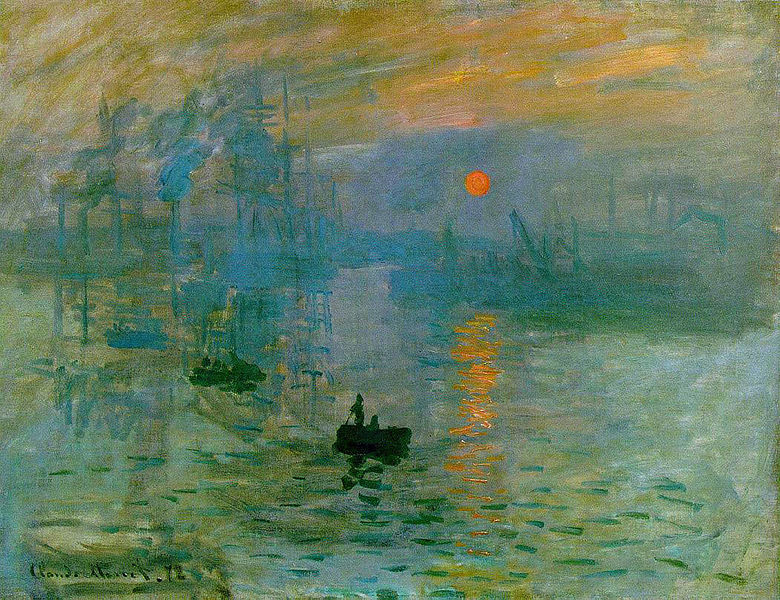
\includegraphics[width=6.67cm]{780px-Claude_Monet_Impression_soleil_levant_1872.jpg}
          \caption{印象·日出(公有领域)}
          \label{fig:impression-soleil-levant}
        \end{figure}
        
        1872年,莫奈以勒阿弗尔的一处风景为背景创作了《印象·日出》\footnote{\textit{Impression, soleil levant}}(图\ref{fig:impression-soleil-levant})。它在1874年第一次印象派画家展上亮相,如今它陈列在巴黎马蒙丹·莫奈美术馆\footnote{Muse Marmottan-Monet}。从这幅画的题目中,艺术评论家路易·勒鲁瓦提出了「印象派」的说法。莫奈有两幅关于林荫大道的画作,一副现在在莫斯科的普希金博物馆中,另一幅在堪萨斯城的纳尔逊-阿特金斯艺术博物馆中。人们从来都不清楚到底哪幅才是1874年展览中展出的,尽管近来人们倾向于认为是在莫斯科的那幅。
        1870年,莫奈与东西厄结婚。1871年,他们搬进了塞纳河\footnote{Seine River}边阿让特伊\footnote{Argenteuil}的一幢房子。正是在这个时期,莫奈创作了大量的作品。1876年,莫奈夫人生病了。1878年3月17日,他们有了另一个儿子,米歇尔\footnote{Michael}。1879年,莫奈夫人死于肺结核。

    \section{后来的日子}
    \esection{Later life}
        
        卡米尔去世后的数个月,伤心欲绝的莫奈为了不再陷入贫困而认真创作了一些19世纪最棒的绘画。19世纪80年代初,他绘制了几组风景和海景作为他在法国乡村生活的记录。这些记录演变成了他的系列画作。
        
        1878年莫奈一家暂时搬到Ernest~Hosched\footnote{1837年 --- 1891年}的房子中居住。他是一个富裕的百货商店老板,并且也是艺术赞助人。那个夏天,这两个家庭分享了在Vtheuil的这套房子。在那之后Ernest~Hosched破产了,并于1878年前往比利时。1879年,东西厄逝世后,莫奈依然居住在那里。Alice~Hoschede决定帮助莫奈抚养他的两个孩子,并带去巴黎,和她自己的六个孩子在一起。1880年他们从巴黎回来了。1881年,他们搬到了普瓦西\footnote{Poissy},但莫奈不喜欢那里。1883年4月,他们搬到了上诺曼底大区厄尔省的Giverny。他种植了一个大花园并在那里完成了他余生的绘画创作。莫奈和Alice~Hoschede在1892年结婚。
    
    \section{在吉维尼}
    \esection{Giverny}
    
        1883年5月初,莫奈和他的家族从本地的一个田主手中租下了一个房子。这个房子座落在Vernon和吉维尼的Gasny。房子中有一个谷仓被用作画室,但也是果园和小花园。房子离本地的学校很近,周围的景观给莫奈的作品提供了很多灵感。随着一家在此劳作,修耆院子,莫奈的作品也被经销商保罗·杜兰德-鲁埃尔越卖越多,他的命运得到了改变。直到1890年11月,莫奈已经买得起他的房子和周边建筑了。十九世纪90年代,莫奈创建了一个温室和他的第二个工作室,那是一个包含天窗的宽敞的建筑。
        
        在十九世纪八十年代和九十年代,莫奈开始了系列绘画创作,即在不同的光线和角度连续画同一个物体。他的第一个系列作品《鲁昂主教座堂》就是在不同的角度和一天中不同的时间来画。1895年,从20个不同角度对大教堂所作的画在迪朗德 --- 吕埃尔\footnote{Gurand-Ruel}画廊展出。此外,他的作品还有稻草堆系列、白杨系列、伦敦议会、塞纳河的早晨、睡莲系列。

        \begin{figure}[h!]
          \begin{minipage}{0.5\textwidth}
              \centering
              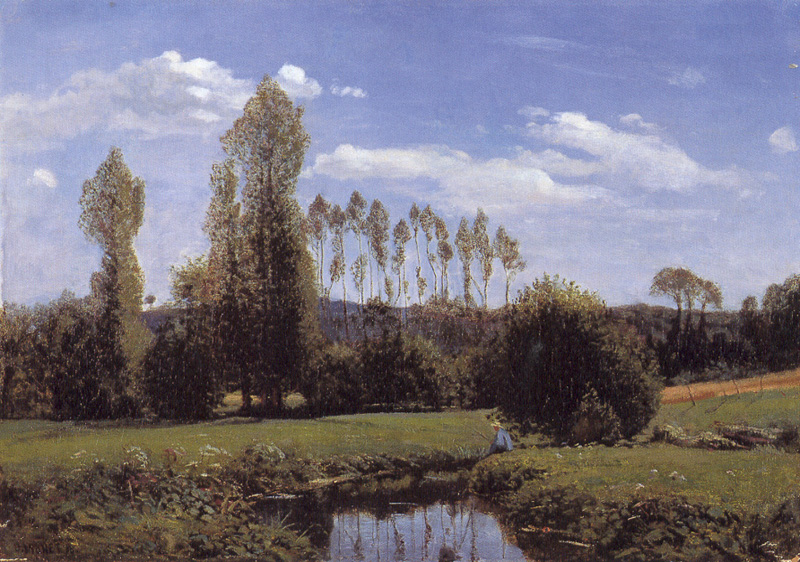
\includegraphics[width=6.67cm]{Monet-Claude_-_View_At_Rouelles_Le_Havre_1858.jpg}
              \caption{\textit{View At Rouelles, Le Havre} (公有领域)}
              \label{fig:view-at-rouelles-le-havre}
          \end{minipage}
          \begin{minipage}{0.5\textwidth}
              \centering
              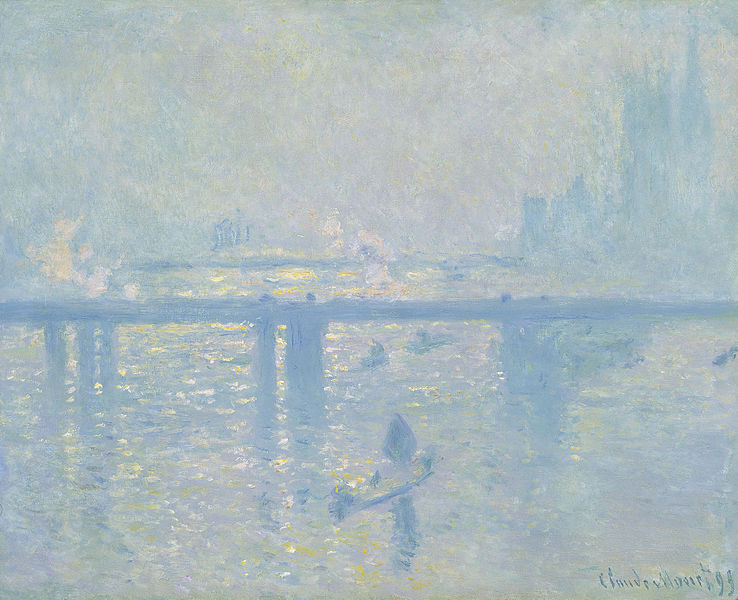
\includegraphics[width=6.67cm]{738px-Charing_Cross_Bridge_Monet.jpg}
              \caption{\textit{Charing Cross Bridge}  (公有领域)}
              \label{fig:charing-cross-bridge}
          \end{minipage}
        \end{figure}
        
        莫奈喜欢绘制受控状态下的自然:他在吉维尼的院子和里面的睡莲,还有桥。他还画了塞纳河的上上下下,产生了如塞纳河上的冰破裂了的画作。他每天给他的园丁写的指示中包含了精确的设计和种植布局,以及购买花卉和植物学书籍。与莫奈的财富增长伴随着的是他的花园的进化。甚至在他雇佣了7名园丁的时候,他依然保留了花园的建筑师。
        
        1883年至1908年间,莫奈在地中海画了许多风景画和海景画。在意大利威尼斯,他画了一系列重要的画作,在伦敦他绘制了两个重要的系列——议会系列和查林十字街大桥系列。他的第二个妻子,Alice,在1911年逝世。他特别喜欢的、娶了Alice的女儿布兰奇的大儿子,于1914年去世。妻子逝世后,布兰奇照顾和关心他。这段时间,莫奈身上出现了白内障的最初迹象。
        
        第一次世界大战期间,他年轻的儿子米歇尔参军,他的朋友、崇拜者乔治·克列孟梭领导法国。莫奈绘制了一系列垂柳树以表达对法国阵亡将士的敬意。1923年,莫奈接受了两次白内障手术,以减小他的画作受到白内障症状的影响:因为白内障影响了他的视力,画作整体偏红。也可能是这样:他在手术后可以看到某些正常人看不见的紫外线,这会影响到他观察到的颜色。在手术后,他甚至重新绘制了他的作品,其中的睡莲(图\ref{fig:water-lilies})更蓝了。


        \begin{figure}[h!]
          \centering
          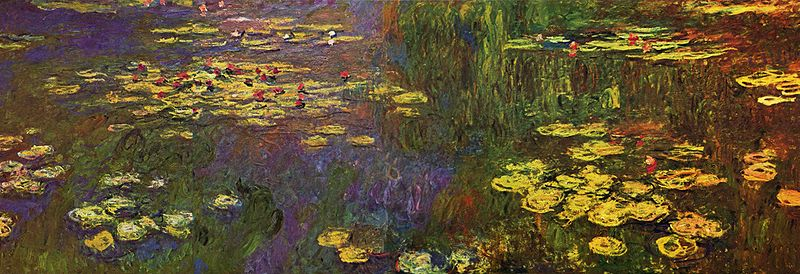
\includegraphics[width=12cm]{800px-Claude_Monet_038.jpg}
          \caption{睡莲(原作属于公有领域,编译版权归Zenodot Verlagsgesellschaft mbH,依GFDL协议使用)}
          \label{fig:water-lilies}
        \end{figure}
        
    \section{逝世}
    \esection{Death}
    
        他于1926年12月5日死于肺癌,享年86岁,下葬于吉维尼教堂的墓地。莫奈坚持葬礼的仪式要简单,因此大约只有五十人出席了他的葬礼。
        
        他的家,他的花园和睡莲由唯一继承人也就是他的儿子米歇尔继承,并于1966年捐赠给法国美术学院。通过莫奈基金会,他的房子和花园在1980年复原后开放参观。除了莫奈的纪念品和他一生中的其他事物,房子中还包含了他收集的日本木刻版画他的房子也是吉维尼两个主要景点之一。

        \begin{figure}[h!]
          \centering
          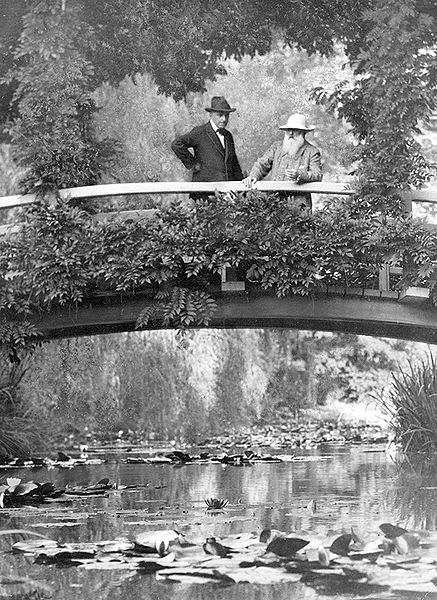
\includegraphics[width=6.67cm]{437px-Monet_in_Garden_New_York_Times_1922.jpg}
          \caption{莫奈在他的花园中。右为莫奈(公有领域)}
          \label{fig:monet-in-gardon}
        \end{figure}

    \section{作品的销售}
    \esection{Posthumous sales}
        
        2004年,莫奈的\textit{the Parliament}和\textit{Effects of Sun in the Fog}在伦敦卖出了超过2000万美元。2006年,英国皇家学报发表文章指出这两幅画作是在泰晤士河上的圣托马斯医院创作的。
    
        他的作品《迪耶普附近的悬崖》被盗两次。一次是在1998年,博物馆的馆长被裁定与两名同伙一起盗窃,因此被判入狱五年零两个月;另一次是在2007年8月,并于2008年找回。他在1873年创作的作品\textit{Le Pont du chemin de fer \`a Argenteuil},描绘了巴黎附近塞纳河上的一座铁路桥。这幅作品2008年5月6日被一个匿名电话竞标者在纽约克里斯蒂拍卖行以4140万美元竞得。在此之前,他的单幅作品售价的最高记录是3650万美元。仅仅几周之后的2008年6月24日,睡莲系列中的\textit{Le bassin aux nymphas}在伦敦佳士得拍出。落锤价是36,500,000英镑\footnote{71,892,376.34美元},算上竞拍费用高达40,921,250英镑\footnote{80,451,178美元},是当时最贵的20幅画作之一。
